\label{Gukena}
\chapter{Gukena}
Los usuarios exigen cualidades al software destinadas a facilitar su trabajo, ahorrar tiempo (de uso y de aprendizaje), evitar y corregir los errores \cite{definicionUsuarioInterfaz}. El cómputo provisorio de los votos en la Universidad Nacional del Comahue se realizaba en forma manual por una persona, encargada de ingresar los datos en una planilla electrónica. Esta persona era responsable de gestionar correctamente los resultados y distribuir los cargos. La forma de trabajo generaba un cuello de botella en la carga de los datos produciendo una demora de varias horas y hasta días en obtener los resultados finales.

Luego de haber analizado las propiedades sensibles que pueden ser afectados al involucrar tecnología en alguna de las etapas dentro del proceso electoral, se desarrolla Gukena con la intención de ayudar y/o acompañar a esta persona responsable. Siempre dentro de las etapas sobre las cuales se corre menos riesgo de corromper la voluntad del votante. Gukena es un sistema responsable de realizar estos cómputos y distribuir la carga de trabajo hacia distintos sitios. Ha sido utilizado con éxito en las últimas elecciones que se desarrollaron en el ámbito de la Universidad Nacional del Comahue, usado a partir del año 2016. Este sistema ayuda a distribuir el trabajo en lo que respecta a la carga de la información de votos, y acorta el tiempo de espera para conocer los resultados provisorios de las elecciones, incluso permite observar resultados parciales en tiempo real.\newline

Una vez que la autoridad de mesa finaliza el recuento y completa el acta en papel,  la información es ingresada en el sistema manualmente desde cualquier computadora o dispositivo móvil con acceso a Internet. Previamente, las autoridades de mesa, recibieron un breve instructivo de carga y un sobre cerrado con usuario y clave para ingresar al sistema. De igual modo, además de esta carga electrónica, el acta en papel es enviada a la Junta Electoral. Con esto, ante cualquier inconveniente que pueda surgir, como la falta de acceso a Internet o cualquier otro,  impidiendo que el acta sea cargada por la autoridad de mesa, la Junta Electoral es quien se responsabiliza en realizar su carga al sistema.

Como segunda etapa, la junta electoral accede al sistema y verifica los datos cargados cotejando con las actas recibidas, permitiendo así resolver cualquier error de carga. 
El proceso de escrutinio finaliza con una última validación, sobre los datos de todas las mesas, a cargo de la secretaria de la Junta Electoral. 

Todo el proceso se encuentra disponible al público generando un ámbito transparente al presenciar y observar los resultados parciales en todo momento, tanto de manera presencial como virtual por medio de una página web abierta.

Algunas ventajas de utilizar el sistema, además de la disminución del tiempo en el proceso de escrutinio, son:
\begin{itemize}
\item Carga distribuida de las actas en el sistema, actas cargadas directamente por el responsable de la misma y sin intermediarios,
\item Resultados accesibles desde cualquier navegador o dispositivo con acceso a internet,
\item Ayudar a comprender mejor los datos de un acta mal redactada o poco legible,
\item Detectar consistencia en el recuento de votos. Contar con doble verificación permite detectar la totalidad de errores y validación de datos durante la carga del acta, ofreciendo mayor seguridad en esos momentos. Como por ejemplo, en casos en que se pretende registrar más votantes que la cantidad de empadronados que contiene la mesa.
\item Distribución de responsabilidades, tanto a nivel de carga de datos sobre distintos sitios, como distribución de roles dentro del sistema electoral como es la carga y validación.
\item Mejora en la visualización y búsqueda de datos cargados dentro del sistema, como es por tipo de cargo o unidad académica, disponible a cualquier persona que acceda a la página de resultados.
\end{itemize}

\section{Análisis}
\subsection{Metodología de desarrollo}
Utilizar una metodología adecuada al momento de un desarrollo es importante para lograr el objetivo del producto final. Existen muchas metodologías tradicionales como ágiles, estas últimas permiten un proceso de desarrollo más rápido con la intención de no afectar la calidad del producto. Una metodología ágil consiste en un desarrollo incremental con iteraciones muy cortas, beneficiando principalmente a proyectos con requisitos cambiantes y con exigencias en los tiempos de desarrollo \cite{canos2012metodologias}. Volcando este concepto dentro del desarrollo de Gukena se puede decir que se utilizó la metodología SCRUM. Cada año representa una iteración (o sprint), donde cada iteración duraba de 4-5 semanas de desarrollo con reuniones cada semana dentro de cada iteración. Las Historias de Usuario son las técnicas para especificar los requisitos del software, estas describen brevemente las características que el sistema debe poseer, requisitos funcionales o no funcionales.
\subsection{Historias de usuario en Gukena}
 Cada historia de usuario establecida en Gukena es comprensible y delimitada para que el equipo conformado pueda llevarla a cabo en unas semanas. A continuación se listan las historias de usuario agrupado por año:\newline
\subsubsection{2015}
\begin{enumerate}
    \item Investigación y aprendizaje sobre el proceso de elecciones en la Universidad Nacional del Comahue, junto al uso del método D'Hondt.
    \item Diseño y modelado de la base de datos utilizando una base de datos relacional.
    \item Preparación ambiente de trabajo, utilizando framework Toba y gestor de base de datos PostgreSQL.
    \item Análisis del archivo de cálculo resultante en las elecciones del corriente año.
    \item Creación de controladores para el formulario de carga de una Autoridad de Mesa.
    \item Creación de controladores para la grilla de mesas con sus estados.
    \item Simulación de carga utilizando los datos del archivo de cálculo recibido de personas participantes en las elecciones de este año.
\end{enumerate}
\subsubsection{2016}
\begin{enumerate}
    \item Análisis y modelado de los datos involucrados en el control de acceso al sistema.
    \item Investigación e integración de seguridad utilizando la herramienta de login que provee el framework Toba
    \item Unión del modelado de datos referidos al control de acceso con la herramienta de login.
    \item Integración con registros de seguimiento sobre actualizaciones en los datos por parte de cada usuario logueado.
    \item Preparación de datos para las elecciones de este año.
    \item Testeo final sobre la funcionalidad en la carga de datos y su resultado final.
\end{enumerate}
\subsubsection{2017}
\begin{enumerate}
    \item Preparación de datos para las elecciones de este año.
    \item Testeo final sobre la funcionalidad en la carga de datos y su resultado final.
    \item Preparación del documento que especifica el Procedimiento de Gukena dentro del marco de elecciones en la Universidad Nacional del Comahue.
\end{enumerate}
\subsubsection{2018}
\begin{enumerate}
    \item Nuevo diseño para las pantallas visibles por el público en general.
    \item Adaptación del sistema para crear archivos con datos que serán consumidos por nuevas pantallas.
    \item Creación de nuevas pantallas.
    \item Procesamiento de los datos para generar los archivos json consumidos por estas nuevas pantallas.
    \item Creación de script encargado de copiar los archivos con los datos procesados entre dos servidores, desde el servidor procesador de los datos del sistema hacia el servidor público visualizador de los datos.
    \item Preparación de datos para las elecciones de este año.
    \item Testeo final sobre la funcionalidad en la carga de datos y su resultado final.
    \item Preparación del ambiente de trabajo, esto involucra ambos servidores junto al script y datos dentro del sistema.
\end{enumerate}
\subsubsection{2019}
\begin{enumerate}
    \item Preparación de datos para las elecciones de este año.
    \item Testeo final sobre la funcionalidad en la carga de datos y su resultado final.
    \item Preparación del ambiente de trabajo, esto involucra ambos servidores junto al script y datos dentro del sistema.
\end{enumerate}

\section{Diseño}

\subsection{Arquitectura}
Gukena se implementó sobre una arquitectura dividida en tres módulos que se relacionan con los diferentes roles que interaccionan con el sistema.
\begin{itemize}
\item Módulo Resultados: muestra los resultados en un servidor web público, para que la comunidad universitaria pueda conocer los resultados a medida que se van cargando los datos.
\item Módulo Autoridad de Mesa: desde cualquier dispositivo con conexión a Internet las Autoridades de Mesa acceden con su usuario y clave para cargar los datos del acta desde el lugar de votación.
\item Módulo Junta Electoral: los integrantes de la junta electoral y la Secretaria realizan un doble chequeo de las actas cargadas por las Autoridades de Mesa en una red interna.
\end{itemize}

La propiedad de usabilidad es importante para que un sistema sea fácil de aprender y de utilizar. Cada uno de estos módulos implican actividades disjuntas dentro del sistema, por lo tanto, para cada rol se le dispuso una interacción distinta con el sistema. \newline
El público en general tiene la necesidad ver los resultados parciales durante el proceso de escrutinio, para cumplir este objetivo se accede a Gukena a través del siguiente link:  \url{https://resultados.uncoma.edu.ar/gukena/}.
Esta página es accesible desde cualquier navegador, contiene un historial de elecciones, categorías de búsqueda de información, gráficos y descripciones explicativas sobre los datos visualizados. Por otro lado, el rol de autoridad de mesa tiene la necesidad de transmitir la información del resultado de su escritinio, por este motivo acceden a \url{https://gukena.fi.uncoma.edu.ar/},
donde se loguean con la información recibida previamente y acceden a una única pantalla con un formulario correspondiente a la mesa escrutada. Por último tenemos al módulo de Junta Electoral quienes necesitan validar y/o corregir la información cargada en el sistema. Acceden al mismo link que una autoridad de mesa con la diferencia que al validar múltiples mesas, el sistema le dispone un listado de todas las mesas, con filtros y categorías para facilitar su búsqueda. Además, cada mesa se encuentra etiquetada con información sobre su estado, es decir, si ya fue cargada por la autoridad de mesa correspondiente o en la espera de su carga. Por cada mesa se le despliega la misma pantalla que se dispone a una autoridad de mesa para que pueda hacer las correcciones necesarias con una acción de validar esta información. Cabe destacar que una autoridad de mesa solo tiene disponible el formulario de carga hasta que envia la información cargada, a partir de ese momento solo puede visualizar el formulario pero no volver a editarlo.\newline

Por otro lado, a nivel técnico Gukena se desarrolló sobre una infraestructura web LAPP como variación a la arquitectura LAMP. Es decir, se implementó sobre un sistema base Linux, servidor web Apache, sistema gestor de base de datos PostgreSQL, y el lenguaje de programación PHP. Siendo todas estas herramientas libres y gratuitas consiguiendo las mismas prestaciones que cualquier herramienta que no sea libre.

\subsection{Seguridad}
Una vulnerabilidad (en términos de informática) es una debilidad o fallo en un sistema de información que pone en riesgo la seguridad de la información pudiendo permitir que un atacante pueda comprometer la integridad, disponibilidad o confidencialidad de la misma \cite{definicionVulnerabilidad}.
Se ha contemplado y evaluado la Seguridad en cada fase  del diseño e implementación del sistema.  La principal amenaza es que se vulnere el enlace con los usuarios que cargan y verifican los datos.  Por esta razón, los tres módulos están publicados en un servidor web Apache a través del protocolo HTTPS para asegurar el enlace. Además, la verificación de la Junta Electoral y la confirmación de la Secretaría se realizan dentro de una red interna. \newline
Además no existe un enlace directo entre los datos del escrutinio cargado al sistema y los datos visualizados por el público. Los datos procesados son depositados en archivos con formato JSON los cuales son actualizados continuamente cada 5 minutos por un script interno y, estos archivos son levantados por la página web para su correcta visualización. Existen muchos tipos de ataques a los datos de un sistema con el fin de obtener información, manipularlos o destruirlos. Podemos nombrar algunos de estos ataques como por ejemplo: accesos no autorizados al sistema o a la base de datos, inyección por SQL, Malware y spear phising, etc. El término Inyección por SQL consiste en la inserción de código SQL por medio de los datos de entrada desde la parte del cliente hacia la aplicación. Es decir, por medio de la inserción de este código el atacante puede modificar las consultas originales que debe realizar la aplicación y ejecutar otras totalmente distintas con la intención de acceder a la herramienta, obtener información de alguna de las tablas o borrar los datos almacenados, entre otras muchas cosas. Al conocer este término se puede ver que debido a que la página utiliza archivos para alimentarse y no realiza consultas SQL directas a la base de datos, este tipo de ataque no es posible. Como mayor daño podría llegar a ser manipular o destruir estos archivos, que luego son reemplazados nuevamente de manera automática por el sistema con los datos reales y correctos. \newline
Otro de los ataques que se nombraron es el acceso no autorizado al sistema con el objetivo de manipular los datos cargados del escrutinio en una mesa en particular, o un conjunto de ellas. Los usuarios con los roles de Autoridad de mesa, Junta Electoral y Secretaría tienen login con nombre de usuario y clave para ingresar al sistema. Esta información es enviada de manera impresa dentro de un sobre cerrado con la instrucción de que la persona encargada del cierre de la mesa de votación lo abra para ingresar al sistema. Además se registra cada acción de inserción y modificación que se realiza en los formularios del sistema en un log general. \newline


\subsection{Proceso de la Elección}


El procedimiendo electoral en la Universidad Nacional del Comahue se rige a través de la Ordenanza Nº1386/13, del Consejo Superior de la Universidad Nacional del Comahue \cite{ordenanzaUncoma}. Luego de varias elecciones exitosas dentro del ámbito, se establece una metodología a utilizar para computar los resultados de actos electorales realizados en el ámbito de la Universidad Nacional del Comahue, utilizando un sistema de escrutinio descentralizado. \newline
El proceso electoral utilizando Gukena se compone de los siguientes pasos:
\begin{itemize}
\item Paso 1: Carga de listas y mesas. Se carga la información de las listas de candidatos oficializadas y las mesas electorales con su respectiva cantidad de empadronados.
\item Paso 2: Se validan los datos cargados en el Sistema. Se corrobora que la información cargada en la Base de Datos del Sistema gukena es la misma que la que fue oficializada por la Junta Electoral.
\item Paso 3: Sobres con usuario. Se arma un sobre para cada mesa que contenga la información del Usuario y la Contraseña para poder acceder al sistema. Ejemplo en la imagen \ref{graf:ejemploSobre}

\begin{figure}[h!]
    \begin{center}
        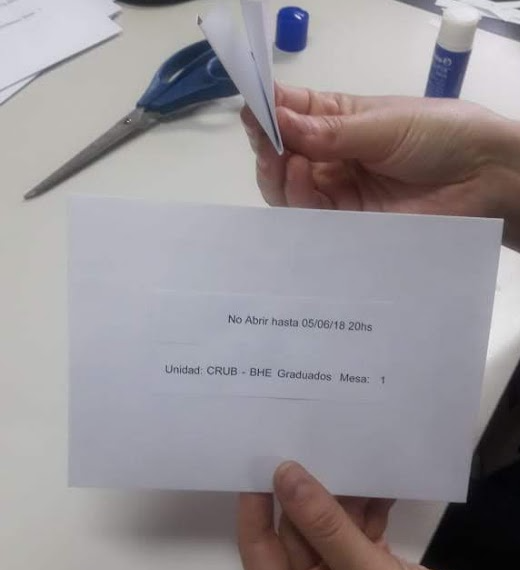
\includegraphics[scale=0.5]{jKz6EB2F9Z.png}
    \end{center}
  \caption{Ejemplo Sobre enviado dentro de la urna de la mesa nº1}
  \label{graf:ejemploSobre}
\end{figure}

\item Paso 4: Envío de material. Se envía a cada dependencia el material necesario para poder llevar a cabo los comicios, incluyendo un breve instructivo de carga para la Autoridad de Mesa y el sobre cerrado nombrado en el paso anterior (que sólo debe ser abierto al momento de cargar el acta en el sistema).
\item Paso 5: El Acto Electoral se lleva a cabo en las fechas fijadas por el cronograma electoral y cumpliendo con lo especificado en la Ordenanza Nº 1386/13.
\item Paso 6: Escrutinio Provisorio de la Mesa. 
Una vez que haya finalizado el Acto Electoral, las Autoridades de Mesa realizan el escrutinio provisorio de los votos obtenidos en su mesa, para luego completar por duplicado el acta en papel con la información obtenida del recuento. Ejemplo de un acta cargada en la imagen \ref{graf:ejemploActa}.

\begin{figure}[h!]
    \begin{center}
        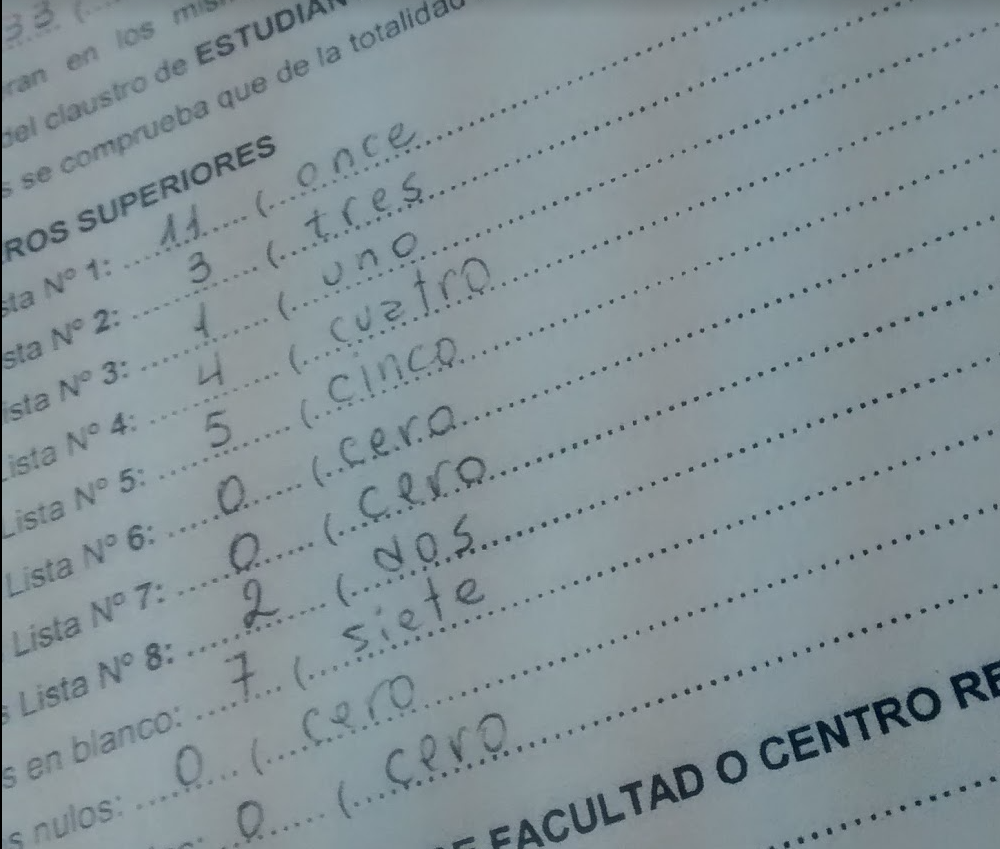
\includegraphics[scale=0.25]{f4P4qmrKXY.png}
    \end{center}
  \caption{Ejemplo Acta en papel completada por una Autoridad de Mesa}
  \label{graf:ejemploActa}
\end{figure}

\item Paso 7: Finalizado el Acto Electoral, se habilita el Sistema Gukena para que pueda ingresar cada Autoridad de mesa.
\item Paso 8: Carga y envío de datos en Gukena. Una vez que haya completado el acta papel, la Autoridad de Mesa carga la información de ésta en el Sistema Gukena. Para esto deben ingresar al mismo utilizando el usuario y contraseña contenidos en el sobre. Ejemplo de la pantalla del login en la imagen \ref{graf:ejemploLogin}.
Cuando los datos del acta son confirmados o enviados por la Autoridad de Mesa, estos datos ya no pueden ser editados por este usuario.

\begin{figure}[h!]
    \begin{center}
        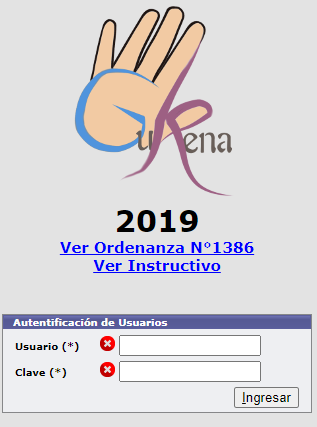
\includegraphics[scale=0.5]{ZJ3mtjmmdZ.png}
    \end{center}
  \caption{Pantalla de login para el módulo Autoridad de Mesa y Junta Electoral}
  \label{graf:ejemploLogin}
\end{figure}

\item Paso 10: La Autoridad de Mesa deposita un ejemplar del acta dentro de la urna antes de cerrarla y otro ejemplar es enviado a la Junta Electoral, enviada por los medios disponibles por la Autoridad de Mesa, por ejemplo fax, email, entre otros. 
\item Paso 11: Primera Validación de datos. La Junta Electoral confirma en el sistema que los datos cargados, por las autoridades de mesa, coinciden con las actas papel recibidas, permitiendo corregir cualquier error ocurrido durante el proceso de carga. Para aquellas actas que, por algún inconveniente, no fueran cargadas por la Autoridad de Mesa, como se especifica en el paso anterior, deben ser cargadas por algún miembro de la Junta Electoral.
\item Paso 12: Segunda Validación de los datos. La Secretaria de la Junta Electoral realiza una segunda validación de las actas ya confirmadas por la Junta, en el caso de encontrar diferencias devuelve el acta a la Junta Electoral para su corrección. Si no hay diferencias, entonces dicha acta queda confirmada en el sistema. Una vez que el acta es confirmada ya no puede ser modificada por ningún miembro de la Junta Electoral.

\end{itemize}

\subsection{Modelo de datos}
La semántica de este problema se representó sobre una base de datos relacional utilizando herramientas de software libre. Se utilizó el Gestor de Base de Datos PostgreSQL sobre un sistema operativo Linux. El modelo de datos representa los conceptos más importantes en un dominio, conociendo el proceso de elección en la Universidad Nacional del Comahue se puede ver que las clases más importantes son: Unidad Electoral, mesas, claustros, actas y las listas oficializadas para cada cargo. En base a estas clases principales tenemos los votos que recibe cada lista postulada que se agrupan por las sedes que conforman cada Unidad Electoral. Además para mantener el histórico de elecciones se tiene la clase de acto electoral manteniendo las fechas de cada elección realizada.\newline
Conociendo el modelo de datos, al momento de una nueva elección es necesario realizar una precarga de datos sobre:
\begin{itemize}
    \item Acto electoral con fecha de la nueva elección, asociando los claustros que votarán y las unidades electorales y sedes participantes
    \item Datos de las mesas: número de mesa, cantidad de empadronados en cada mesa, claustro al que pertenece.
    \item Listas oficializadas para cada claustro y el cargo al que se postula
    \item Usuarios habilitados a ingresar al sistema
\end{itemize}

\begin{figure}[h!]
  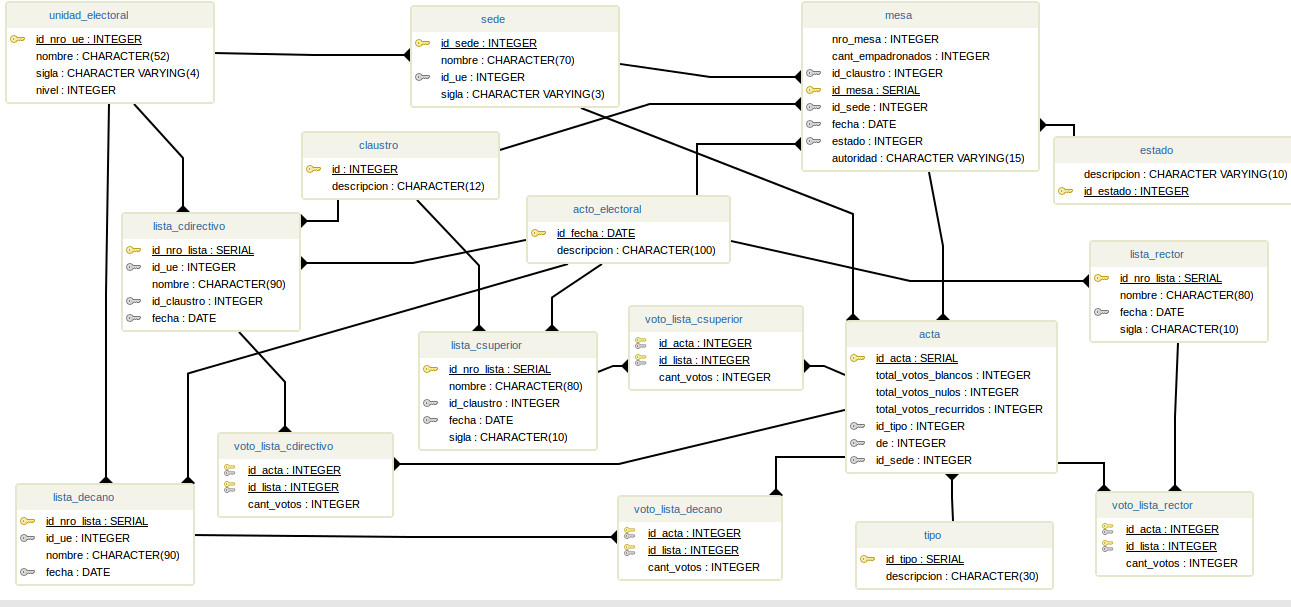
\includegraphics[width=\textwidth]{gu_kena_diagramaBD.jpg}
  \caption{Diagrama de clases}
  \label{graf:diagramaBD}
\end{figure}

Este modelo de datos representado en la Figura \ref{graf:diagramaBD} es el almacenamiento principal del sistema, es decir, la carga de datos por parte de las autoridades de mesa y Junta Electoral y, el procesamiento de los resultados impacta sobre esta fuente de datos. \newline
Sin embargo, se podría decir que la visualización de los resultados al público en general dispone de una segunda fuente de datos de Gukena conformada por archivos en formato JSON. Estos archivos son actualizados durante el escrutinio cada 5 minutos. La estructura de estos archivos está formada por:
\begin{itemize}
    \item data (lista, sigla , total de votos, sede)
    \begin{itemize}
        \item lista (String)
        \item sigla (String)
        \item total de votos (int)
        \item sede (int)
    \end{itemize}
    \item columns (field , title)
    \begin{itemize}
        \item field (String)
        \item title (String)
    \end{itemize}
    \item titulo (String)
    \item labels (String)
    \item total (int)
    \item fecha (datetime)
    \item enviados y confirmadas (String)
    \item titulo\_grafico (String)
\end{itemize}
Esta información es consumida por cada pantalla visualizado por el público. Para reconocer que archivo debe consumir cada pantalla se aplicó una notación conformada por \textbf{nombreCargo} + \textbf{siglaUnidadElectoral} + \textbf{nombreClaustro} + \textbf{".json"} en el nombre de cada archivo. En la tabla \ref{tab:formatoJSON} se representa este formato.

\begin{table}[htbp]
\begin{center}
\begin{tabular}{|l|l|l|}
\hline
Categoria\_ & Unidad\_Electoral & \_ Claustro.json\\
\hline \hline 
R(Rector) & Todo(Universidad) & T(Total)\\ \hline
D(Decano) & ASMA & D(Docentes)\\ \hline
CD(Consejo Directivo) & AUZA & E(Estudiantes)\\ \hline
CS(Consejo Superior) & CRUB & G(Graduados)\\ \hline
-& CUZA & N(No Docentes) \\ \hline
-& ESCM &- \\ \hline
-& FACA &- \\ \hline
-& FACE &- \\ \hline
-& FADE &- \\ \hline
-& FACA &- \\ \hline
-& FAEA &- \\ \hline
-& FAHU &- \\ \hline
-& FAIF &- \\ \hline
-& FAIN &- \\ \hline
-& FALE &- \\ \hline
-& FAME &- \\ \hline
-& FATA &- \\ \hline
-& FATU &- \\ \hline
\end{tabular}
\end{center}
\caption{Nombre de archivos JSON}
\label{tab:formatoJSON}
\end{table}

\section{Desarrollo}
Gukena ha sido construido por el Grupo de Desarrollo Euclides \cite{euclides} que está integrado por un conjunto de no docentes, estudiantes avanzados y docentes de la Facultad de Informática en la Universidad Nacional del Comahue y funciona bajo la dirección de la Subsecretaría de Tecnologías de la Información de la misma Universidad. El sistema se desarrolló durante los meses de abril a junio a partir del 2015 y los años siguientes, integrándose mejoras evolutivas en cada año.

Para el desarrollo del sistema se utiliza el modelo de ciclo de vida iterativo e incremental, basado en la metodología Scrum, para promover un proceso de construcción ágil y una comunicación fluida con el cliente y, conseguir los beneficios del sistema de forma incremental. En 2015 una primera versión se utilizó para validar las planillas usadas hasta el momento, en 2016 y 2017 se empleó el sistema de forma completa.  En 2018 fue la primera vez que se utilizó en una elección completa considerando los cuatro claustros y la elección de Rector, Decano, Consejeros Directivos y Superiores. Este año se aplicaron mejoras sobre las pantallas accesibles por el público en general que permiten ver los resultados parciales en tiempo real, junto a un histórico de elecciones. Esta mejora fue bien aceptada por el público y permitió a los medios de comunicación tener un acceso rápido.

En la construcción, diseño e implementación de Gukena se utilizan solamente herramientas de software libre. Se usa el ambiente desarrollo web SIU Toba \cite{toba}, que es desarrollado por el consorcio SIU para soluciones del Sistema Universitario Nacional. Esta herramienta  permite crear sistemas transaccionales en forma rápida, utilizando tecnología web open-source y apunta a agilizar el proceso de construcción y el mantenimiento de los mismos, a través de la reducción de tareas repetitivas, se permite al equipo de desarrollo enfocar su actividad en la lógica del dominio.  El ambiente integra el lenguaje de programación PHP, servidor web Apache, sistema operativo Linux y bases de datos PostgreSQL, entre otros.

Se trabaja utilizando con la filosofía del desarrollo opensource, para contribuir a mejorar el mantenimiento del sistema. Los fuentes son de licencia libre y acceso público, se encuentran disponibles en el repositorio \cite{github} con la intensión  de que la comunidad de desarrolladores, investigadores, y comunidad de la Universidad puedan acceder al software y analizarlo.

El ambiente de desarrollo web SIU Toba está basado en el patrón arquitectónico MVC (Model, View, Controller), el cual separa los datos de una aplicación, la interfaz de usuario y la lógica de control en tres componentes distintos. Este patrón permite la separación de conceptos, características que buscan facilitar la tarea de desarrollo de aplicaciones y su posterior mantenimiento. Por lo tanto, este tipo de arquitectura permitió dividir tareas de desarrollo dentro del grupo Euclides y permitió facilitar su evolución por cada año de experiencia. \newline
De manera genérica los componentes de MVC se pueden describir como:
\begin{itemize}
    \item Model (Modelo): Es la representación de la información con la cual el sistema opera y gestiona todos los accesos a dicha información. En este contexto, el Modelo permite guardar y consultar los datos del escrutinio final por cada mesa. Además este componente se encargó de aplicarle las fórmulas necesarias para conseguir el resultado provisorio y/o final de la distribución de escaños. Otra información importante que gestionó fue el log de actualizaciones sobre estos datos, esto permite satisfacer las propiedades de auditabilidad, ya que se registran las actualizaciones por parte de las autoridades de mesa y personal de la Junta Electoral autorizada.
    \item View (Vista): Presenta el Modelo de una manera adecuada para interactuar, es decir, la interfaz de usuario. Se encarga de la representación visual de los datos que gestiona el Modelo. Gukena dispuso una vista por cada módulo de interacción. De manera tal que una autoridad de mesa solo accede a un formulario de carga, una persona autorizada de la Junta Electoral accede a un listado de mesas a validar, y por último una vista más gráfica para el módulo de Resultados. Este componente tiene la responsabilidad de satisfacer las propiedades de usabilidad del sistema.
    \item Controller (Controlador): Responde a eventos e invoca peticiones al Modelo, se encarga de controlar las acciones del usuario y de solicitar los datos al Modelo para comunicarselos a la vista. En Gukena, el Controlador suministró los datos mediante dos vias, una de ellas es la comunicación directa entre Vista y Modelo para los módulos de Autoridad de Mesa y Junta Electoral, sin embargo, para el módulo de Resultados el controlador 'empaquetaba' los datos y los depositaba en archivos JSON, los cuales eran el origen de datos para este módulo.
\end{itemize}
Como se puede ver, una de las ventajas de esta arquitectura MVC es que permite separar los componentes de una aplicación dependiendo de la repsonsabilidad que tienen. Esto respeta el principio de la responsabilidad única.

\section{Testing}